\documentclass[11pt,a4paper]{article}
\usepackage{amsmath}
\usepackage{amssymb}
\usepackage{array}
\usepackage{extarrows}
\usepackage{float}
\usepackage[margin=2.5cm]{geometry}
\usepackage[unicode=true,pdftex,pdfa]{hyperref}
\usepackage[capitalise,noabbrev,nameinlink]{cleveref}
\usepackage[utf8]{inputenc}
\usepackage{latexsym}
\usepackage{listings}
\usepackage{mathpazo} % nice fonts
\usepackage{mathtools}
\usepackage{microtype}
\usepackage[colon]{natbib}
\usepackage[toc,page]{appendix}
%%
%% Package `semantic` can be used for writing inference rules.
%%
\usepackage{semantic}
\usepackage{slashed}
\usepackage{stmaryrd}
\usepackage[colorinlistoftodos,prependcaption,textsize=tiny]{todonotes}

\hypersetup{
  pdftitle={Specification of the Blockchain Layer},
  breaklinks=true,
  bookmarks=true,
  colorlinks=false,
  linkcolor={blue},
  citecolor={blue},
  urlcolor={blue},
  linkbordercolor={white},
  citebordercolor={white},
  urlbordercolor={white}
}
\floatstyle{boxed}
\restylefloat{figure}

%% Setup for the semantic package
\setpremisesspace{20pt}

\DeclareMathOperator{\dom}{dom}
\DeclareMathOperator{\range}{range}

%%
\newcommand{\powerset}[1]{\mathbb{P}~#1}
\newcommand\Set[2]{\left\{\,#1\mid#2\,\right\}}
\newcommand{\restrictdom}{\lhd}
\newcommand{\subtractdom}{\mathbin{\slashed{\restrictdom}}}
\newcommand{\restrictrange}{\rhd}
\newcommand{\union}{\cup}
\newcommand{\unionoverride}{\mathbin{\underrightarrow\cup}}
\newcommand{\uniondistinct}{\uplus}
\newcommand{\var}[1]{\mathit{#1}}
\newcommand{\fun}[1]{\mathsf{#1}}
\newcommand{\type}[1]{\mathsf{#1}}
\newcommand{\pp}[1]{\mathsf{#1}}
\newcommand{\size}[1]{\left| #1 \right|}
\newcommand{\trans}[2]{\xlongrightarrow[\textsc{#1}]{#2}}
\newcommand{\seqof}[1]{#1^{*}}
\newcommand{\serialised}[1]{\llbracket \var{#1} \rrbracket}

\newcommand{\leteq}{\ensuremath{\mathrel{\mathop:}=}}

% Partial and total function aliases
\newcommand{\totalf}{\to}
\newcommand{\partialf}{\mapsto}

%%
%% Types
%%
\newcommand{\Hash}{\type{Hash}}  % hashes of various things, including blocks
\newcommand{\Slot}{\type{Slot}}
\newcommand{\SlotCount}{\type{SlotCount}}
\newcommand{\BlockIx}{\type{BlockIx}}
\newcommand{\Block}{\type{Block}}
\newcommand{\DCert}{\type{DCert}}
\newcommand{\Queue}{\type{Q}}
\newcommand{\Tx}{\type{Tx}}

\newcommand{\VKey}{\type{VKey}}
\newcommand{\VKeyGen}{\type{VKey_G}}
\newcommand{\Sig}{\type{Sig}}
\newcommand{\Data}{\type{Data}}
\newcommand{\DelegState}{\type{DIState}}

\newcommand{\ProtParams}{\type{PParams}} % protocol parameters
\newcommand{\ProtPm}{\ensuremath{\type{Ppm}}}
\newcommand{\maxblocksize}{\pp{maxBlockSize}}
\newcommand{\maxheadersize}{\pp{maxHeaderSize}}

\newcommand{\Nothing}{\Diamond}

%%
%% Function and relation names
%%
\newcommand{\bsizename}{bSize}
\newcommand{\bhdrsizename}{bHeaderSize}
\newcommand{\verifyname}{verify}

\newcommand{\isebbname}{bIsEBB}
\newcommand{\bcertsname}{bCerts}
\newcommand{\bhsigname}{bhSig}
\newcommand{\bhissuername}{bhIssuer}

%%
%% Functions and relations
%%
\newcommand{\verify}[3]{\fun{\verifyname} ~ #1 ~ #2 ~ #3}
\newcommand{\bsize}[1]{\fun{\bsizename} ~ #1}
\newcommand{\bhdrsize}[1]{\fun{\bhdrsizename} ~ #1}
\newcommand{\delegation}[2]{\fun{\delegationname} ~ #1 ~ #2}
\newcommand{\signmap}[1]{\fun{\signmapname} ~ #1}
\newcommand{\qrestr}[2]{\fun{\qrestrname} ~ #1 ~ #2}
\newcommand{\trimix}[2]{\fun{\trimixname} ~ #1 ~ #2}
\newcommand{\incixmap}[3]{\fun{\incixmapname} ~ #1 ~ #2 ~ #3}

\newcommand{\hashofblock}[1]{\fun{\hashofblockname} ~ #1}
\newcommand{\blocksizelimit}[2]{\fun{\blocksizelimitname} ~ #1 ~ #2}
\newcommand{\isebb}[1]{\fun{\isebbname} ~ #1}
\newcommand{\bcerts}[1]{\fun{\bcertsname} ~ #1}
\newcommand{\bhsig}[1]{\fun{\bhsigname} ~ #1}
\newcommand{\bhissuer}[1]{\fun{\bhissuername} ~ #1}

\newcommand{\qpop}[1]{\fun{\qpopname} ~ #1}
\newcommand{\qhead}[1]{\fun{\qheadname} ~ #1}
\newcommand{\qpush}[1]{\fun{\qpushname} ~ #1}


% A type alias for a map from a genesis block verification key to a queue of indices
\newcommand{\mapqueue}{\mathcal{Q}}
% comments
\newcommand{\marko}[1]{\todo[size=\small, color=yellow!40, inline]{Marko: #1}}

\begin{document}

\title{Specification of the Blockchain Layer}

\author{Marko Dimjašević \\ Nicholas Clarke}

\date{May 2, 2019}

\maketitle

\begin{abstract}
  This documents defines inference rules for operations on a blockchain as a
  specification of the blockchain layer of Cardano in the Byron release and in
  a transition to the Shelley release.
  %
  In particular, a block validity definition is given, which is accompanied by
  small-step operational semantics inference rules.
\end{abstract}

\section*{List of Contributors}
\label{acknowledgements}

Damian Nadales, Yun Lu.

\tableofcontents
\listoffigures

\section{Introduction}
\label{sec:introduction}

The idea behind this document is to formalise what it means for a new block to
be added to the blockchain to be valid.
%
The scope of the document is the Byron release and a transition phase to the
Shelley release of the Cardano blockchain platform.


Unless a new block is valid, it cannot be added to the blockchain and thereby
extend it.
%
This is needed for a system that is subscribed to the blockchain and keeps a
copy of it locally.
%
In particular, this document gives a formalisation that should be
straightforward to implement in a programming language, e.g., in Haskell.

This document is intended to be read in conjunction with \cite{byron_ledger_spec},
which covers the payload carried around in the blockchain. Certain of the
underlying systems and types defined will rely on definitions in that document.

\section{Preliminaries}
\label{sec:preliminaries}

\begin{description}
\item[Powerset] Given a set $\type{X}$, $\powerset{\type{X}}$ is the set of all
  the subsets of $X$.
\item[Sequence] Given a set $\type{X}$, $\seqof{\type{X}}$ is a sequence
  having elements taken from $\type{X}$.
  %
  The empty sequence is denoted by $\epsilon$, and given a sequence $\Lambda$,
  $\Lambda; x$ is the sequence that results from appending
  $x \in \type{X}$ to $\Lambda$.
  %
  Furthermore, $\epsilon$ is an identity element for sequence joining:
  $\epsilon; x = x; \epsilon = x$.
\item[Dropping on sequences] Given a sequence $\Lambda$,
  $\Lambda \shortdownarrow n$ is the sequence that is obtained after removing
  (dropping) the first $n$ elements from $\Lambda$. If $n \leq 0$ then
  $\Lambda \shortdownarrow n = \Lambda$.
\item[Appending with a moving window] Given a sequence $\Lambda$, we define
  $$\Lambda ;_w x \leteq (\Lambda; x) \shortdownarrow (\size{\Lambda} + 1 - w)$$
\item[Filtering on sequences] Given a sequence $\Lambda$, and a predicate $p$
  on the elements of $\Lambda$, $\fun{filter}~p~\Lambda$ is the sequence that
  contains all the elements of $\Lambda$ that satisfy $p$, in the same order
  they appear on $\Lambda$.
\item[Option type] An option type in type $A$ is denoted as $A^? = A + \Nothing$. The
  $A$ case corresponds to a case when there is a value of type $A$ and the $\Nothing$
  case corresponds to a case when there is no value.
\item[Union override] The union override operation is defined in
  Figure~\ref{fig:unionoverride}.
  %
  \begin{figure}
    \begin{align*}
      \var{K} \restrictdom \var{M}
      & = \{ i \mapsto o \mid i \mapsto o \in \var{M}, ~ i \in \var{K} \}
      & \text{domain restriction}
      \\
      \var{K} \subtractdom \var{M}
      & = \{ i \mapsto o \mid i \mapsto o \in \var{M}, ~ i \notin \var{K} \}
      & \text{domain exclusion}
      \\
      \var{M} \restrictrange \var{V}
      & = \{ i \mapsto o \mid i \mapsto o \in \var{M}, ~ o \in \var{V} \}
      & \text{range restriction}
      \\
      & \unionoverride \in (A \mapsto B) \to (A \mapsto B) \to (A \mapsto B)
      & \text{union override}\\
      & d_0 \unionoverride d_1 = d_1 \cup (\dom d_1 \subtractdom d_0)
    \end{align*}
    \caption{Definition of the Union Override Operation}
    \label{fig:unionoverride}
  \end{figure}
\item[Pattern matching in premises] In the inference-rules premises use
  $\var{patt} = \var{exp}$ to pattern-match an expression $\var{exp} $ with a
  certain pattern $\var{patt}$. For instance, we use $\Lambda'; x = \Lambda$ to
  be able to deconstruct a sequence $\Lambda$ in its last element, and prefix.
  If an expression does not match the given pattern, then the premise does not
  hold, and the rule cannot trigger.
\item[Maps and partial functions] $A \mapsto B$ denotes a \textbf{partial
    function} from $A$ to $B$, which can be seen as a map (dictionary) with
  keys in $A$ and values in $B$. Given a map $m \in A \mapsto B$, notation
  $a \mapsto b \in m$ is equivalent to $m~ a = b$.
\end{description}

\subsection{Sets}
\label{sec:sets}

There are several standard sets used in the document:
%
\begin{description}
\item[Booleans] The set of booleans is denoted with $\mathbb{B}$ and has two
  values, $\mathbb{B} = \{\bot, \top\}$.
\item[Natural numbers] The set of natural numbers is denoted with
  $\mathbb{N}$ and defined as $\mathbb{N} = \{0, 1, 2, \dots\}$.
\end{description}

\section{Update interface}

\newcommand{\bupdprop}[1]{\fun{bUpdProp}\ #1}
\newcommand{\bupdvotes}[1]{\fun{bUpdVotes}\ #1}
\newcommand{\bprotver}[1]{\fun{bProtVer}\ #1}
\newcommand{\bendorsment}[1]{\fun{bEndorsment}\ #1}

\newcommand{\UpdatePayload}{\type{UpdatePayload}}
% Imported definitions

\newcommand{\UPIEnv}{\type{UPIEnv}}
\newcommand{\UPIState}{\type{UPIState}}
\newcommand{\UProp}{\type{UProp}}
\newcommand{\Vote}{\ensuremath{\type{Vote}}}
\newcommand{\ProtVer}{\ensuremath{\type{ProtVer}}}

We define a general update interface to abstract over the various update state
transitions which happen when a new block is processed. Figure
\ref{fig:defs:bupi} defines the type of signals used for this system. Figure
\ref{fig:rules:bupi} defines the rules for this system. The two rules handle the
cases where there is or is not an update proposal contained within the block.

\begin{figure}[ht]
  \emph{Update interface signals}
  \begin{equation*}
    \UpdatePayload =
    \left(
      \begin{array}{r@{~\in~}lr}
        \var{mprop} & \UProp^{?} & \text{possible update proposal}\\
        \var{votes} & \seqof{\Vote} & \text{votes for update proposals}\\
        \var{end} & (\VKey \times \ProtVer) & \text{protocol version endorsment}
      \end{array}
    \right)
  \end{equation*}

  \caption{Update interface processing types and functions}
  \label{fig:defs:bupi}
\end{figure}

\begin{figure}[ht]
  \emph{Update interface processing transitions}
  \begin{equation*}
    \_ \vdash \var{\_} \trans{bupi}{\_} \var{\_} \subseteq
    \powerset (\UPIEnv \times \UPIState \times \UpdatePayload \times \UPIState)
  \end{equation*}
  \caption{Update interface processing transition-system types}
  \label{fig:ts-types:bupi}
\end{figure}

\begin{figure}[ht]
  \begin{equation*}
    \inference
    { \Gamma \vdash \var{us}
      \trans{\hyperlink{byron_ledger_spec_link}{upireg}}{\var{prop}} \var{us'}
      \\
      \Gamma \vdash \var{us'}
      \trans{\hyperlink{byron_ledger_spec_link}{upivotes}}{\var{votes}} \var{us''}
      &
      \Gamma \vdash \var{us''}
      \trans{\hyperlink{byron_ledger_spec_link}{upiend}}{\var{end}} \var{us'''}
    }
    {
      \Gamma \vdash
      {\var{us}}
      \trans{bupi}
      {
        \left(
          \begin{array}{l}
            \var{prop} \\
            \var{votes} \\
            \var{end}
          \end{array}
        \right)
      }
      {\var{us'''}}
    }
  \end{equation*}
  \vspace{20pt}
  \begin{equation*}
    \inference
    { \Gamma \vdash \var{us}
      \trans{\hyperlink{byron_ledger_spec_link}{upivotes}}{\var{votes}} \var{us'}
      &
      \Gamma \vdash \var{us'}
      \trans{\hyperlink{byron_ledger_spec_link}{upiend}}{\var{end}} \var{us''}
    }
    {
      \Gamma \vdash \var{us}
      \trans{bupi}{
        \left(
          \begin{array}{l}
            \Nothing \\
            \var{votes} \\
            \var{end}
          \end{array}
        \right)
      }
      \var{us''}
    }
  \end{equation*}
  \caption{Update interface processing rules}
  \label{fig:rules:bupi}
\end{figure}

\clearpage
\section{Permissive BFT}

The majority of this specification is concerned with the processing of the
\textit{ledger}; that is, the content (contained in both the block header and
the block body). In addition, however, we must also concern ourselves with the
protocol used to transmit the blocks and whether, according to that protocol, we
may validly extend the chain with a new block (assuming that block forms a valid
extension to the chain under the ledger rules).

Cardano's planned evolution can be split into roughly three eras:
\begin{description}
\item[Byron/Ouroboros] In the Byron/Ouroboros era, the Ouroboros (\cite{ouroboros})
  protocol is used to control who is eligible to issue a block, using a stake
  distribution mediated by heavyweight delegation certificates. The Byron
  payload includes such things as VSS and payloads verified by individual
  signatures.
\item[Handover] In the handover era, blocks will be issued according to
  Ouroboros BFT (\cite{ouroboros_bft}). The Byron payload will be retained, although
  parts of will be superfluous.
\item[Shelley/Praos] In the Shelley/Praos era, blocks will be issued according
  to the Ouroboros Praos (\cite{ouroboros_praos}) protocol, with stake distribution
  determined according to the new delegation design in \cite{delegation_design}.
\end{description}

During the handover era (as described in this document), while blocks will be
issued according to Ouroboros BFT, they will be validated according to a variant
known as Permissive BFT. This is designed such that it will successfully
validate blocks issued both under Ouroboros and under Ouroboros BFT (with a high
probability - see Appendix \ref{apdx:calculating-t}).

This section therefore will describe the section of the rules concerned with the
Permissive BFT protocol. Note that all of these are concerned only with the
block header, since the block body is entirely concerned with the ledger.

\subsection{Counting signed blocks}

\newcommand{\BSCEnv}{\type{BSCEnv}}
\newcommand{\BSCState}{\type{BSCState}}

To guard against the compromise of a minority of the genesis keys, we require
that in the rolling window of the last $k$ blocks, where $k$ is the chain
stability parameter, the number of blocks signed by keys that $sk_s$ delegated
to is no more than a threshold $k \cdot t$, where $t$ is a constant that will
be picked in the range $1/5 \leq t \leq 1/4$. Initial research suggests setting
$t=0.22$ as a good value. Specifically, given $k=2160$, we would allow a single
genesis key to issue (via delegates) $475$ blocks (since
$2160 \cdot 0.22 = 475.2$), but a $476^{\text{th}}$ block would be rejected.
See Appendix \ref{apdx:calculating-t} for the background on this value. The
abstract constant (nullary functions) related to the protocol are defined in
\cref{fig:defs:proto-abstract-funcs}.

\begin{figure}[ht]
  \emph{Abstract functions}
  %
  \begin{equation*}
    \begin{array}{r@{~\in~}lr}
      k & \mathbb{N} & \text{chain stability parameter}\\
      t & \left[\frac{1}{5}, \frac{1}{4}\right] & \text{block signature count threshold}\\
      \fun{dms} & \DelegState \totalf (\VKeyGen \mapsto \VKey) & \text{delegation-state delegation-map}
    \end{array}
  \end{equation*}

  \caption{Protocol abstract functions}
  \label{fig:defs:proto-abstract-funcs}
\end{figure}


Figure \ref{fig:rules:sigcnt} gives the rules for signature counting. We verify
that the key that delegates to the signer of this block has not already signed
more than its allowed threshold of blocks. If there are no delegators for the
given key, or if there is more than one delegator, the rule will fail to trigger.
%
We then update the sequence of signers, and drop those elements that fall
outside the size of the moving window ($k$).

\begin{figure}[ht]
  \emph{Block signature count environments}
  \begin{equation*}
    \BSCEnv =
    \left(
      \begin{array}{r@{~\in~}lr}
        \var{ds} & \DelegState & \text{delegation state} \\
      \end{array}
    \right)
  \end{equation*}

  \emph{Block signature count transitions}
  \begin{equation*}
    \_ \vdash \var{\_} \trans{sigcnt}{\_} \var{\_} \subseteq
    \powerset (\BSCEnv \times \seqof{\VKeyGen} \times \VKey \times \seqof{\VKeyGen})
  \end{equation*}
  \caption{Block signature count transition-system types}
  \label{fig:ts-types:sigcnt}
\end{figure}

\begin{figure}[ht]
  \begin{equation*}
    \inference
    {
      \{\var{vk_g}\} \leteq \dom{((\fun{dms} ~ \var{ds}) \restrictrange \{\var{vk_d}\})}
      & \var{sgs'} \leteq \var{sgs};_k {vk_g} &
      \size{\fun{filter}~(=\var{vk_g})~\var{sgs'}} \leq k \cdot t \\
    }
    {
      \var{ds}
      \vdash
      {\var{sgs}}
      \trans{sigcnt}{\var{vk_d}}
      {\var{sgs'}}
    }
   \label{eq:rule:sigcnt}
 \end{equation*}
 \caption{Block signature count rules}
 \label{fig:rules:sigcnt}
\end{figure}

\clearpage

\subsection{Permissive BFT Header Processing}

\newcommand{\PBFTEnv}{\type{PBFTEnv}}
\newcommand{\PBFTState}{\type{PBFTState}}

\newcommand{\Bhead}{\type{BlockHeader}}
\newcommand{\Bhtosign}{\type{BHToSign}}

\newcommand{\bhslotname}{bhSlot}
\newcommand{\bhslot}[1]{\fun{\bhslotname}\ #1}
\newcommand{\bhhashname}{bhHash}
\newcommand{\bhhash}[1]{\fun{\bhhashname}\ #1}
\newcommand{\bhprevhashname}{bhPrevHash}
\newcommand{\bhprevhash}[1]{\fun{\bhprevhashname}\ #1}
\newcommand{\bhtosignname}{bhToSign}
\newcommand{\bhtosign}[1]{\fun{\bhtosignname}\ #1}

During PBFT processing of the block header, we do the following:
\begin{enumerate}
 \item We check that the current block is being issued for a slot later than
    that of the last block issued.
  \item We check that the current block is being issued for a slot no later than
    the current slot (as determined by the system clock).
  \item We verify that the block signer is the current delegate of at least one
    of the authorised genesis keys.
  \item We check that the previous block hash contained in the block header
    corresponds to the known hash of the previous block.
  \item We check that the header signature correctly verifies the ``signed''
    content of the header.
  \item Finally, we verify and update the state according to the signature count rules.
  \end{enumerate}
  \begin{figure}[ht]
  \emph{Abstract types}
  %
  \begin{equation*}
    \begin{array}{r@{~\in~}lr}
      bh & \Bhead & \text{Block header}
    \end{array}
  \end{equation*}
  %
  \emph{Abstract functions}
  %
  \begin{equation*}
    \begin{array}{r@{~\in~}lr}
      \fun{\bhprevhashname} & \Bhead \totalf \Hash & \text{previous header hash} \\
      \fun{\bhhashname} & \Bhead \totalf \Hash & \text{header hash} \\
      \fun{\bhsigname} & \Bhead \totalf \Sig & \text{block signature} \\
      \fun{\bhissuername} & \Bhead \totalf \VKey & \text{block issuer} \\
      \fun{\bhslotname} & \Bhead \totalf \Slot & \text{slot for which this block is issued}
    \end{array}
  \end{equation*}
  \caption{Permissive BFT types and functions}
  \label{fig:defs:pbft}
\end{figure}

\begin{figure}[ht]
  \emph{Permissive BFT environments}
  \begin{equation*}
    \PBFTEnv =
    \left(
      \begin{array}{r@{~\in~}lr}
        \var{ds} & \DelegState & \text{delegation state} \\
        \var{s_{last}} & \Slot & \text{slot for which the last known block was issued} \\
        \var{s_{now}} & \Slot & \text{current slot} \\
      \end{array}
    \right)
  \end{equation*}

  \emph{Permissive BFT states}
  \begin{equation*}
    \PBFTState =
    \left(
      \begin{array}{r@{~\in~}lr}
        \var{h} & \Hash & \text{Tip header hash} \\
        \var{sgs} & \seqof{\VKeyGen} & \text{Last signers}
      \end{array}
    \right)
  \end{equation*}
  \emph{Permissive BFT transitions}
  \begin{equation*}
    \_ \vdash \var{\_} \trans{pbft}{\_} \var{\_} \subseteq
    \powerset (\PBFTEnv \times \PBFTState \times \Bhead \times \PBFTState)
  \end{equation*}
  \caption{Permissive BFT transition-system types}
  \label{fig:ts-types:pbft}
\end{figure}

\begin{figure}[ht]
  \begin{equation*}
    \inference
    {
      \var{vk_d} \leteq \bhissuer{bh} & \var{s} \leteq \bhslot{bh}
      \\ \var{s} > \var{s_{last}} & \var{s} \leq \var{s_{now}}
      \\ \bhprevhash{bh} = \var{h} & \verify{vk_d}{\serialised{\bhtosign{bh}}}{(\bhsig{bh})}
      \\
      ds
      \vdash
      \var{sgs} \trans{\hyperref[fig:rules:sigcnt]{sigcnt}}{\var{vk_d}} \var{sgs'}
      \\
    }
    {
      \left(
        {\begin{array}{c}
           \var{ds} \\
           \var{s_{last}} \\
           \var{s_{now}} \\
         \end{array}}
     \right)
     \vdash
     \left(
       {\begin{array}{c}
          \var{h} \\
          \var{sgs}
        \end{array}}
    \right)
    \trans{pbft}{\var{bh}}
    \left(
      {\begin{array}{c}
         \bhhash{bh} \\
         \var{sgs}'
       \end{array}}
   \right)
 }
\end{equation*}
\caption{Permissive BFT rules}
\label{fig:rules:pbft}
\end{figure}


\clearpage

\section{Epoch transitions}

\newcommand{\Epoch}{\type{Epoch}}

\newcommand{\ETState}{\type{ETState}}
\newcommand{\ETEnv}{\type{ETEnv}}

\newcommand{\sepochname}{sEpoch}
\newcommand{\sepoch}[1]{\fun{\sepochname}\ #1}

During each block transition, we must determine whether that block sits on an
epoch boundary and, if so, carry out various actions which are done on that
boundary. In the BFT era, the only computation carried out at the epoch boundary
is the update of protocol versions.

We rely on a function $\fun{\sepochname}$, whose type is given in
\cref{fig:defs:epoch}, to determine the epoch corresponding to a given slot.
%
We do not provide an implementation for such function in this specification,
but in practice a possible way of implementing such function is to rely on map
from the epochs to their corresponding length (given in number of slots they
contain). Such a map would also be required by the database layer to find the
requisite epoch file to look up a given block. We envision that an
implementation may of course choose a more compact representation for this
partial function that only records the changes in epoch length, rather than
storing a length for each epoch.
%
In addition, we rely on abstract constant (nullary function) $\var{ngk}$, which
determines the number of genesis keys.

It is also worth noticing that in the Byron era, the number of slots per-epoch
is fixed to $10 \cdot k$, where $k$ is the chain stability parameter.

Figure \ref{fig:rules:epoch} determines when an epoch change has occurred and
updates the update state to the correct version.

\begin{figure}[ht]
  \emph{Abstract functions}
  %
  \begin{equation*}
    \begin{array}{r@{~\in~}lr}
      \fun{\sepochname}
      & \Slot \totalf \Epoch
      & \text{epoch containing this slot} \\
      \var{ngk} & \mathbb{N} & \text{number of genesis keys}\\
    \end{array}
  \end{equation*}

  \caption{Epoch transition types and functions}
  \label{fig:defs:epoch}
\end{figure}

\begin{figure}[ht]
  \emph{Epoch transition environments}
  \begin{align*}
    & \ETEnv
      = \left(
      \begin{array}{r@{~\in~}lr}
        \var{dms} & \VKeyGen \mapsto \VKey & \text{delegation map}\\
        \var{e_c} & \Epoch & \text{Current epoch}
      \end{array}\right)
  \end{align*}

  \emph{Epoch transition states}
  \begin{equation*}
    \ETState =
    \left(
      \begin{array}{r@{~\in~}lr}
        \var{us} & \UPIState & \text{update interface state}
      \end{array}
    \right)
  \end{equation*}

  \emph{Epoch transition transitions}
  \begin{equation*}
    \_ \vdash \var{\_} \trans{epoch}{\_} \var{\_} \subseteq
    \powerset (\ETEnv \times \ETState \times \Slot \times \ETState)
  \end{equation*}
  \caption{Epoch transition transition-system types}
  \label{fig:ts-types:epoch}
\end{figure}

\begin{figure}[ht]
  \begin{equation*}
    \inference
    {
      \var{e_c} \geq \sepoch{s}
    }
    {
      {\left(
        \begin{array}{l}
          \var{dms}\\
          \var{e_c}
        \end{array}
      \right)}
      \vdash
      {
        \left(
          {\begin{array}{c}
             \var{us}
           \end{array}
         }
       \right)
     }
     \trans{epoch}{s}
     {
       \left(
         {\begin{array}{c}
            \var{us}
          \end{array}
        }
      \right)
    }
  }
\end{equation*}
\vspace{20pt}
\begin{equation*}
  \inference
  {
    \var{e_c} < \sepoch{s}
    &
    s\vdash \var{us} \trans{\hyperlink{byron_ledger_spec_link}{upiec}}{} \var{us'}
  }
  {
    {\left(
      \begin{array}{l}
        \var{dms}\\
        \var{e_c}
      \end{array}
    \right)}
    \vdash
    {
      \left(
        {\begin{array}{c}
           \var{us}
         \end{array}
       }
     \right)
   }
   \trans{epoch}{s}
   {
     \left(
       {\begin{array}{c}
          \var{us'}
        \end{array}
      }
    \right)
  }
}
\end{equation*}
\caption{Epoch transition rules}
\label{fig:rules:epoch}
\end{figure}

\clearpage

\section{Block processing}
\label{sec:block-processing}

\newcommand{\BHEnv}{\type{BHEnv}}
\newcommand{\BHState}{\type{BHState}}

\newcommand{\BBEnv}{\type{BBEnv}}
\newcommand{\BBState}{\type{BBState}}

\newcommand{\bheadname}{bHead}
\newcommand{\bhead}[1]{\fun{\bheadname}\ #1}
\newcommand{\bupdpayloadname}{bUpdPayload}
\newcommand{\bupdpayload}[1]{\fun{\bupdpayloadname}\ #1}

\newcommand{\bslotname}{bSlot}
\newcommand{\bslot}[1]{\fun{\bslotname}\ #1}

\newcommand{\butxo}[1]{\fun{bUtxo}\ #1}

% Imported definitions
\newcommand{\UTxO}{\type{UTxO}}
\newcommand{\UTxOState}{\type{UTxOState}}
\newcommand{\DIEnv}{\type{DIEnv}}
\newcommand{\DIState}{\type{DIState}}

We delineate here between processing the header and body of a block. It's useful
to make this distinction since we may process headers ahead of the
block body, and we have less context available to process headers - in
particular, we must be able to process block headers without the recent history
of block bodies.

\begin{figure}[ht]
  \emph{Abstract types}
  %
  \begin{equation*}
    \begin{array}{r@{~\in~}lr}
      b & \Block & \text{block} \\
      h & \Hash   & \text{hash} \\
      \var{data} & \Data    & \text{data}
    \end{array}
  \end{equation*}
  %
  %
  \emph{Abstract functions}
  %
  \begin{equation*}
    \begin{array}{r@{~\in~}lr}
      \fun{\bsizename} & \Block \totalf \mathbb{N} & \text{block size in bytes} \\
      \fun{\verifyname} & \VKey \times \Data \times \Sig & \text{verification relation} \\
    \end{array}
  \end{equation*}
  \caption{Basic Block-related Types and Functions}
  \label{fig:block-defs}
\end{figure}

\subsection{Block header processing}

Figure \ref{fig:ts-types:bhead} gives the transition system types for block
header processing. The $\maxheadersize{}$ protocol parameter is defined in
\cite{byron_ledger_spec}. The header state contains the current update state
and historical epoch length map, which must be updated along the epoch
boundary. Figure \ref{fig:rules:bhead} gives the corresponding transition
rules. During header processing we verify the following things:

\begin{enumerate}
  \item We compute whether this block is the first block in a new epoch.
    If so, we apply the epoch transition updates. Unlike other cases, we use the
    resulting update state in all downstream verification for this block, since
    the epoch transition is not contingent on the block itself, but simply a
    recognition that this is a block in a new epoch.
  \item We verify that the block header does not exceed the maximum size
    specified in the protocol parameters.
\end{enumerate}

\begin{figure}[ht]
  \emph{Abstract types}
  %
  \begin{equation*}
    \begin{array}{r@{~\in~}lr}
      bh & \Bhead & \text{block header} \\
      bts & \Bhtosign & \text{part of the block header which must be signed}
    \end{array}
  \end{equation*}
  %
  \emph{Abstract functions}
  %
  \begin{equation*}
    \begin{array}{r@{~\in~}lr}
      \fun{\bheadname} & \Block \totalf \Bhead & \text{block header} \\
      \fun{\bhdrsizename} & \Bhead \totalf \mathbb{N} & \text{block header size in bytes}
    \end{array}
  \end{equation*}
  \caption{Block header processing types and functions}
  \label{fig:defs:bhead}
\end{figure}

\begin{figure}[ht]
  \emph{Block header processing environments}
  \begin{align*}
    & \BHEnv
      = \left(
      \begin{array}{r@{~\in~}lr}
        \var{dms} & \VKeyGen \mapsto \VKey & \text{delegation map}\\
        \var{s_{last}} & \Slot & \text{slot of the last seen block}
      \end{array}\right)
  \end{align*}

  \emph{Block header processing states}
  \begin{equation*}
    \BHState =
    \left(
      \begin{array}{r@{~\in~}lr}
        \var{us} & \UPIState & \text{update state}
      \end{array}
    \right)
  \end{equation*}
  \emph{Block header processing transitions}
  \begin{equation*}
    \var{\_} \vdash \var{\_} \trans{bhead}{\_} \var{\_} \subseteq
    \powerset (\BHEnv \times \BHState \times \Bhead \times \BHState)
  \end{equation*}
  \caption{Block header processing transition-system types}
  \label{fig:ts-types:bhead}
\end{figure}

\begin{figure}[ht]
  \begin{equation*}
    \inference
    {
      {\left(
        \begin{array}{l}
          \var{dms}\\
          \sepoch{s_{last}}\\
        \end{array}
      \right)}
      \vdash
      {\left(
          \begin{array}{l}
            us
          \end{array}
        \right)}
      \trans{\hyperref[fig:rules:epoch]{epoch}}{\bslot{b}}
      {\left(
          \begin{array}{l}
            us'
          \end{array}
        \right)}
      \\
      \\ \maxheadersize \mapsto \var{s_{max}} \in \fun{pps}~\var{us'} & \bhdrsize{bh} \leq \var{s_{max}}
    }
    {
      {\left(
        \begin{array}{l}
          \var{dms}\\
          \var{s_{last}}
        \end{array}
        \right)}
      \vdash
      \left(
        {\begin{array}{c}
           \var{us}
         \end{array}}
     \right)
     \trans{bhead}{\var{bh}}
     \left(
       {\begin{array}{c}
          \var{us'}
        \end{array}}
    \right)
  }
\end{equation*}
\caption{Block header processing rules}
\label{fig:rules:bhead}
\end{figure}

\clearpage

\subsection{Block body processing}

During processing of the block body, we perform two main functions:
verification of the body integrity using the proofs contained in the block
header, and update of the various state components. These rules are given in
\cref{fig:rules:bbody}, where the types and the functions used there are
defined in \cref{fig:ts-types:bbody}. The UTxO, delegation, and update state as
well as the $\maxblocksize{}$ protocol parameter are defined in
\cite{byron_ledger_spec}.

Verification is done independently for the three components of the body payload:
UTxO, delegation and update. Each of these three has a hash in the block
header. Note that Byron-era block payload also has an additional component: the
VSS payload. This part of the block is unnecessary during the BFT era, and hence
we do not verify it.

In addition to block verification, we also process the three components of the
payload; UTxO, delegation and update.

\begin{figure}[ht]
  \emph{Abstract functions}
  %
  \begin{equation*}
    \begin{array}{r@{~\in~}lr}
      \fun{bUtxo} & \Block \totalf (\Tx \times \powerset{(\VKey \times \Sig)}) & \text{block UTxO payload} \\
      \fun{\bcertsname} & \Block \totalf \seqof{\DCert}
                                         & \text{block certificates} \\
      \fun{bUpdProp} & \Block \totalf \UProp^{?} & \text{block update proposal payload} \\
      \fun{bUpdVotes} & \Block \totalf \seqof{\Vote} & \text{block update votes payload} \\
      \fun{bProtVer} & \Block \totalf \ProtVer & \text{block protocol version} \\
      \fun{bhUtxoHash} & \Bhead \totalf \Hash & \text{UTxO payload hash} \\
      \fun{bhDlgHash} & \Bhead \totalf \Hash & \text{delegation payload hash} \\
      \fun{bhUpdHash} & \Bhead \totalf \Hash & \text{update payload hash} \\
      \fun{hash} & \type{Data} \totalf \Hash & \text{hash function} \\
    \end{array}
  \end{equation*}
  \emph{Derived functions}
  \begin{equation*}
    \begin{array}{rlr}
      \fun{bEndorsment} & \in \Block \to \ProtVer \times \VKey & \text{Protocol version endorsment} \\
      \bendorsment{b} & = (\bprotver{b}, (\bhissuername \cdot \bheadname) ~ b)\\
      \fun{\bslotname} & \in \Block \to \Slot & \text{Slot for which this block is being issued} \\
      \bslot{b} & = (\bhslotname \cdot \bheadname)~b \\
      \fun{\bupdpayloadname} & \in \Block \to (\UProp^{?}\times\seqof{\Vote}) & \text{Block update payload} \\
      \bupdpayload{b} & = (\bupdprop{b},~\bupdvotes{b})
    \end{array}
  \end{equation*}
  \caption{Block body processing types and functions}
  \label{fig:defs:bbody}
\end{figure}

\begin{figure}[ht]
  \emph{Block body processing environments}
  \begin{equation*}
    \BBEnv =
    \left(
      \begin{array}{r@{~\in~}lr}
        \var{pps} & \ProtParams & \text{protocol parameters} \\
        \var{e_n} & \Epoch & \text{epoch we are currently processing blocks for} \\
        \var{utxo_0} & \UTxO & \text{genesis UTxO}
      \end{array}
    \right)
  \end{equation*}

  \emph{Block body processing states}
  \begin{equation*}
    \BBState =
    \left(
      \begin{array}{r@{~\in~}lr}
        \var{utxoSt} & \UTxOState & \text{UTxO state} \\
        \var{ds} & \DIState & \text{delegation state} \\
        \var{us} & \UPIState & \text{update interface state}
      \end{array}
    \right)
  \end{equation*}

  \emph{Block body processing transitions}
  \begin{equation*}
    \_ \vdash \var{\_} \trans{bbody}{\_} \var{\_} \subseteq
    \powerset (\BBEnv \times \BBState \times \Block \times \BBState)
  \end{equation*}
  \caption{Block body processing transition-system types}
  \label{fig:ts-types:bbody}
\end{figure}

\begin{figure}[ht]
  \begin{equation*}
    \inference
    { \maxblocksize \mapsto \var{b_{max}} \in \var{pps} && \bsize{b} \leq \var{b_{max}} \\
      \var{bh} \leteq \bhead{b} & \var{vk_d} \leteq \bhissuer{\var{bh}} \\
      \fun{hash}~(\butxo{b}) = \fun{bhUtxoHash}~\var{bh} &
      \fun{hash}~(\bcerts{b}) = \fun{bhDlgHash}~\var{bh} \\
      \fun{hash}~(\bupdpayload{b}) = \fun{bhUpdHash}~\var{bh}\\~\\
      {\left(
          \begin{array}{l}
            \bslot{b} \\
            \fun{dms}~ ds
          \end{array}
        \right)}
      \vdash \var{us} \trans{\hyperref[fig:rules:bupi]{bupi}}{
        {\left(
            \begin{array}{l}
              \bupdprop{b} \\
              \bupdvotes{b} \\
              \bendorsment{b}
            \end{array}
          \right)}
      } \var{us'}
      \\
      {\left(
          \begin{array}{l}
            \dom{(\fun{dms}~ ds)} \\
            \var{e_n}\\
            \bslot{b}
          \end{array}
        \right)}
      \vdash \var{ds} \trans{\hyperlink{byron_ledger_spec_link}{deleg}}{\bcerts{b}} \var{ds'} &
      {\left(
          \begin{array}{l}
            \var{utxo_0} \\
            \var{pps}
          \end{array}
        \right)}
      \vdash \var{utxoSt}
        \trans{\hyperlink{byron_ledger_spec_link}{utxows}}{\butxo{b}} \var{utxoSt'} \\
    }
    {
      \left(
        {\begin{array}{l}
           \var{pps} \\
           \var{e_n} \\
           \var{utxo_0}
         \end{array}}
     \right)
     \vdash
     {
       \left(
         {\begin{array}{c}
            \var{utxoSt} \\
            \var{ds} \\
            \var{us}
          \end{array}}
      \right)
    }
    \trans{bbody}{\var{b}}
    {
      \left(
        {\begin{array}{c}
           \var{utxoSt'} \\
           \var{ds'} \\
           \var{us'}
         \end{array}}
     \right)
   }
 }
\end{equation*}
\caption{Block body processing rules}
\label{fig:rules:bbody}
\end{figure}

\clearpage

\section{Blockchain Extension}
\label{sec:chain-extension}

\newcommand{\CEEnv}{\type{CEEnv}}
\newcommand{\CEState}{\type{CEState}}

Figure \ref{fig:rules:chain-extension} captures the central chain extension
rule. This has two variants, depending on whether the block in question is an
epoch boundary block. Epoch boundary blocks are not required during the BFT era,
but whilst they are not distributed, epoch boundary blocks must still be
processed since their hash forms part of the chain. Since we do not care about
the contents of an epoch boundary block, we check that it does not exceed some
suitably large size, and otherwise simply update the header hash to the block
hash.

If the block is not an epoch boundary block, then we process both the header and
body according to the rules in figures \ref{fig:rules:bhead} and
\ref{fig:rules:bbody} respectively.

\begin{figure}[ht]
  \emph{Abstract functions}
  %
  \begin{equation*}
    \begin{array}{r@{~\in~}lr}
      \fun{\isebbname} & \Block \totalf \mathbb{B} & \text{epoch boundary block check} \\
      \fun{pps} & \UPIState \totalf \ProtParams & \text{update-state protocol-parameters}
    \end{array}
  \end{equation*}
  \caption{Blockchain Extension Types and Functions}
  \label{fig:defs:chain-extension}
\end{figure}

\begin{figure}[ht]
  \emph{Chain extension environments}
  \begin{equation*}
    \CEEnv
    = \left(
      \begin{array}{r@{~\in~}lr}
        \var{s_{now}} & \Slot & \text{current slot} \\
        \var{utxo_0} & \UTxO & \text{genesis UTxO}
      \end{array}\right)
  \end{equation*}


  \emph{Chain extension states}
  \begin{equation*}
    \CEState =
    \left(
      \begin{array}{r@{~\in~}lr}
        \var{s_{last}} & \Slot & \text{slot of the last seen block} \\
        \var{sgs} & \seqof{\VKeyGen} & \text{last signers}\\
        \var{h} & \Hash & \text{current block hash} \\
        \var{utxoSt} & \UTxO & \text{UTxOState} \\
        \var{ds} & \DIState & \text{delegation state}\\
        \var{us} & \UPIState & \text{update interface state} \\
      \end{array}
    \right)
  \end{equation*}

  \emph{Chain extension transitions}
  \begin{equation*}
    \_ \vdash \var{\_} \trans{chain}{\_} \var{\_} \subseteq
    \powerset (\CEEnv \times \CEState \times \Block \times \CEState)
  \end{equation*}

  \caption{Blockchain extension transition-system types}
  \label{fig:ts-types:chain-extension}
\end{figure}

\begin{figure}
  \begin{equation*}
    \inference
    { \isebb{b} & \bsize{b} \leq 2^{21} &
       \var{h'} \leteq \bhhash{(\bhead b)}
    }
    {
     \left(
       {\begin{array}{l}
       \var{s_{now}} \\
       \var{utxo_0}
         \end{array}}
     \right)
     \vdash
     \left(
       {\begin{array}{c}
          \var{s_{last}} \\
          \var{sgs} \\
          \var{h} \\
          \var{utxoSt} \\
          \var{ds} \\
          \var{us}
        \end{array}}
    \right)
    \trans{chain}{b}
    \left(
      {\begin{array}{c}
         \var{s_{last}} \\
         \var{sgs} \\
         \var{h'} \\
         \var{utxoSt} \\
         \var{ds} \\
         \var{us}
       \end{array}}
   \right)
 }
\end{equation*}
\vspace{30pt}
\begin{equation*}
  \inference
  {
    \neg\isebb{b} \\~\\
    {
      \begin{array}{r@{~\vdash~}l}
        {\left(
        \begin{array}{l}
          \fun{dms}~\var{ds}\\
          \var{s_{last}}
        \end{array}
        \right)}
        &
        \left(
          {\begin{array}{c}
             \var{us}
           \end{array}
        }\right)
        \trans{\hyperref[fig:rules:bhead]{bhead}}{\bhead{b}}
        \left(
        {\begin{array}{c}
           \var{us'}
         \end{array}}
        \right)\\
        \left(
        {\begin{array}{l}
           \var{ds} \\
           \var{s_{last}} \\
           \var{s_{now}} \\
         \end{array}}
        \right)
        &
        \left(
          {\begin{array}{c}
             \var{h} \\
             \var{sgs}
           \end{array}}
        \right)
        \trans{\hyperref[fig:rules:pbft]{pbft}}{\bhead{b}}
        \left(
        {\begin{array}{c}
           \var{h'} \\
           \var{sgs}'
         \end{array}}
        \right)\\
        {\left(
        \begin{array}{l}
          \fun{pps} ~  us' \\
          \sepoch{(\bslot{b})} \\
          \var{utxo_0}
        \end{array}
        \right)}
        &
        {\left(
          {\begin{array}{c}
             \var{utxoSt} \\
             \var{ds} \\
             \var{us'}
           \end{array}}
        \right)}
        \trans{\hyperref[fig:rules:bbody]{bbody}}{b}
        {\left(
          {\begin{array}{c}
             \var{utxoSt'} \\
             \var{ds'} \\
             \var{us''}
           \end{array}}
        \right)}
      \end{array}
    }
  }
  {
     \left(
      {\begin{array}{l}
         \var{s_{now}} \\
         \var{utxo_0}
       \end{array}}
     \right)
     \vdash
     \left(
       {\begin{array}{c}
          \var{s_{last}} \\
          \var{sgs} \\
          \var{h} \\
          \var{utxoSt} \\
          \var{ds} \\
          \var{us}
        \end{array}}
    \right)
    \trans{chain}{b}
    \left(
      {\begin{array}{c}
         \var{\bslot{b}} \\
         \var{sgs'} \\
         \var{h'} \\
         \var{utxoSt'} \\
         \var{ds'} \\
         \var{us''}
       \end{array}}
    \right)
  }
\end{equation*}
\caption{Blockchain extension rules}
\label{fig:rules:chain-extension}
\end{figure}
\clearpage
\bibliographystyle{plainnat}
\bibliography{references}
\begin{appendices}
  \section{Calculating the $t$ parameter}
  \label{apdx:calculating-t}

  We originally give the range of $t$ as between $\frac{1}{5}$ and $\frac{1}{4}$.
  The upper bound here is to reduce the possible number of malicious blocks; if
  two of the genesis keys are comprimised, the attackers may not be able to
  produce a longer chain than the honest participants. The lower bound is required
  to prevent a situation in which a chain produced under the initial Ouroboros
  setting produces a chain which, according to the new BFT semantics, is invalid.

  In order to determine the best value of $t$, we must consider the likelihood of
  such an invalid chain being produced by the old procedure of randomly selecting
  the slot leaders for each slot. Given the Cardano chain is still federated, the
  likelihood of this happening is the same for each of the 7 stakeholders, and we
  may model the number of selected slots within a $k$-slot window $X$ as a binomial
  distribution $X \sim \mathrm{B}\left(k, \frac{1}{7}\right)$.

  In each epoch of size $n$ blocks, there are $n-k+1$ such $k$-block windows.
  Boole's inequality gives us that the likelihood of exceeding the threshold in
  any one of these windows is bounded above by the sum of the likelihoods for each
  window. We may thus consider that the probability of a given stakeholder
  violating the threshold in an epoch to be bounded by

  $$(n-k+1)\cdot P(X > t*k)$$

  Appealing to Boole's inequality again, we may multiply this by the number of
  epochs and the number of stakeholders to give a bound for the likelihood of
  generating an invalid chain.

  Figure \ref{fig:calculating-t} gives the bound on the likelihood of threshold
  violation for $t$ in our plausible range: from this we can see that the
  likelihood decreases to a negligible level around $0.21$, and so we choose the
  value of $t=0.22$, giving an upper bound on the likelihood around $6e-10$.
  Increasing $t$ beyond this point gives no decrease in the likelihood of
  violation.

  \begin{figure}[ht]
    \begin{center}
      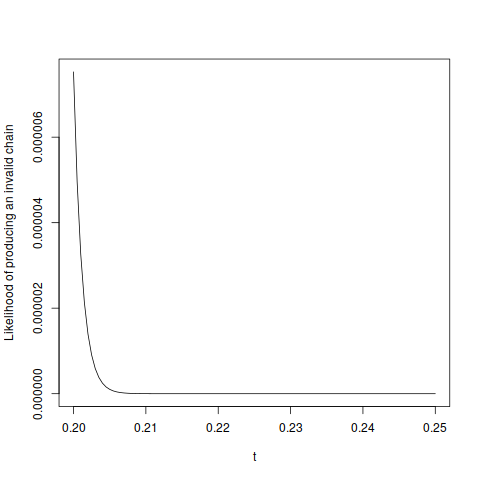
\includegraphics[scale=0.5]{calculating-t.png}
    \end{center}
    \caption{Probability of generating an invalid chain for values of $t\in\left[
        \frac{1}{4}, \frac{1}{5} \right]$.}
    \label{fig:calculating-t}
  \end{figure}

\end{appendices}
\end{document}


%%% Local Variables:
%%% mode: latex
%%% TeX-master: t
%%% LaTeX-command: "nix-shell --run make"
%%% End:
